% Created by tikzDevice version 0.12.3.2 on 2022-02-15 11:22:56
% !TEX encoding = UTF-8 Unicode
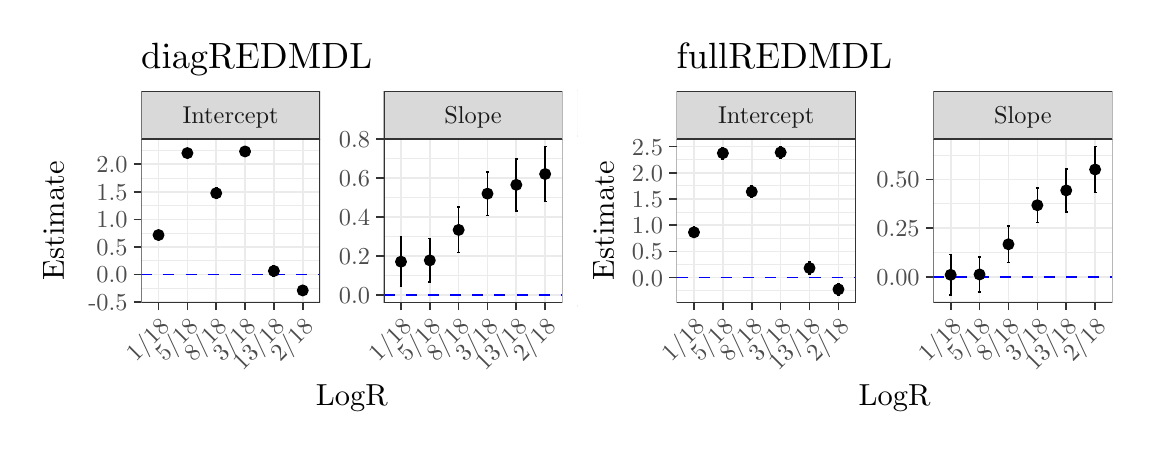
\begin{tikzpicture}[x=1pt,y=1pt]
\definecolor{fillColor}{RGB}{255,255,255}
\path[use as bounding box,fill=fillColor,fill opacity=0.00] (0,0) rectangle (397.48,144.54);
\begin{scope}
\path[clip] (  0.00,  0.00) rectangle (397.48,144.54);
\definecolor{drawColor}{RGB}{255,255,255}
\definecolor{fillColor}{RGB}{255,255,255}

\path[draw=drawColor,line width= 0.6pt,line join=round,line cap=round,fill=fillColor] (  0.00, -0.00) rectangle (397.48,144.54);
\end{scope}
\begin{scope}
\path[clip] ( 34.16, 43.96) rectangle (200.03,105.31);
\definecolor{fillColor}{RGB}{255,255,255}

\path[fill=fillColor] ( 34.16, 43.96) rectangle (200.03,105.31);
\definecolor{drawColor}{gray}{0.92}

\path[draw=drawColor,line width= 0.3pt,line join=round] ( 34.16, 48.42) --
	(200.03, 48.42);

\path[draw=drawColor,line width= 0.3pt,line join=round] ( 34.16, 58.25) --
	(200.03, 58.25);

\path[draw=drawColor,line width= 0.3pt,line join=round] ( 34.16, 68.07) --
	(200.03, 68.07);

\path[draw=drawColor,line width= 0.3pt,line join=round] ( 34.16, 77.90) --
	(200.03, 77.90);

\path[draw=drawColor,line width= 0.3pt,line join=round] ( 34.16, 87.73) --
	(200.03, 87.73);

\path[draw=drawColor,line width= 0.3pt,line join=round] ( 34.16, 97.55) --
	(200.03, 97.55);

\path[draw=drawColor,line width= 0.6pt,line join=round] ( 34.16, 53.34) --
	(200.03, 53.34);

\path[draw=drawColor,line width= 0.6pt,line join=round] ( 34.16, 63.16) --
	(200.03, 63.16);

\path[draw=drawColor,line width= 0.6pt,line join=round] ( 34.16, 72.99) --
	(200.03, 72.99);

\path[draw=drawColor,line width= 0.6pt,line join=round] ( 34.16, 82.81) --
	(200.03, 82.81);

\path[draw=drawColor,line width= 0.6pt,line join=round] ( 34.16, 92.64) --
	(200.03, 92.64);

\path[draw=drawColor,line width= 0.6pt,line join=round] ( 34.16,102.46) --
	(200.03,102.46);

\path[draw=drawColor,line width= 0.6pt,line join=round] ( 50.21, 43.96) --
	( 50.21,105.31);

\path[draw=drawColor,line width= 0.6pt,line join=round] ( 76.96, 43.96) --
	( 76.96,105.31);

\path[draw=drawColor,line width= 0.6pt,line join=round] (103.71, 43.96) --
	(103.71,105.31);

\path[draw=drawColor,line width= 0.6pt,line join=round] (130.47, 43.96) --
	(130.47,105.31);

\path[draw=drawColor,line width= 0.6pt,line join=round] (157.22, 43.96) --
	(157.22,105.31);

\path[draw=drawColor,line width= 0.6pt,line join=round] (183.97, 43.96) --
	(183.97,105.31);
\definecolor{drawColor}{RGB}{0,0,255}

\path[draw=drawColor,line width= 0.6pt,dash pattern=on 4pt off 4pt ,line join=round] ( 34.16, 53.34) -- (200.03, 53.34);
\definecolor{drawColor}{RGB}{0,0,0}
\definecolor{fillColor}{RGB}{0,0,0}

\path[draw=drawColor,line width= 0.4pt,line join=round,line cap=round,fill=fillColor] ( 50.21, 70.32) circle (  1.96);

\path[draw=drawColor,line width= 0.4pt,line join=round,line cap=round,fill=fillColor] (183.97, 48.94) circle (  1.96);

\path[draw=drawColor,line width= 0.4pt,line join=round,line cap=round,fill=fillColor] (130.47,100.30) circle (  1.96);

\path[draw=drawColor,line width= 0.4pt,line join=round,line cap=round,fill=fillColor] ( 76.96,100.01) circle (  1.96);

\path[draw=drawColor,line width= 0.4pt,line join=round,line cap=round,fill=fillColor] (103.71, 85.56) circle (  1.96);

\path[draw=drawColor,line width= 0.4pt,line join=round,line cap=round,fill=fillColor] (157.22, 56.93) circle (  1.96);

\path[draw=drawColor,line width= 0.6pt,line join=round] ( 48.87, 72.21) --
	( 51.55, 72.21);

\path[draw=drawColor,line width= 0.6pt,line join=round] ( 50.21, 72.21) --
	( 50.21, 68.44);

\path[draw=drawColor,line width= 0.6pt,line join=round] ( 48.87, 68.44) --
	( 51.55, 68.44);

\path[draw=drawColor,line width= 0.6pt,line join=round] (182.64, 51.13) --
	(185.31, 51.13);

\path[draw=drawColor,line width= 0.6pt,line join=round] (183.97, 51.13) --
	(183.97, 46.75);

\path[draw=drawColor,line width= 0.6pt,line join=round] (182.64, 46.75) --
	(185.31, 46.75);

\path[draw=drawColor,line width= 0.6pt,line join=round] (129.13,102.52) --
	(131.80,102.52);

\path[draw=drawColor,line width= 0.6pt,line join=round] (130.47,102.52) --
	(130.47, 98.08);

\path[draw=drawColor,line width= 0.6pt,line join=round] (129.13, 98.08) --
	(131.80, 98.08);

\path[draw=drawColor,line width= 0.6pt,line join=round] ( 75.62,102.15) --
	( 78.30,102.15);

\path[draw=drawColor,line width= 0.6pt,line join=round] ( 76.96,102.15) --
	( 76.96, 97.86);

\path[draw=drawColor,line width= 0.6pt,line join=round] ( 75.62, 97.86) --
	( 78.30, 97.86);

\path[draw=drawColor,line width= 0.6pt,line join=round] (102.38, 87.79) --
	(105.05, 87.79);

\path[draw=drawColor,line width= 0.6pt,line join=round] (103.71, 87.79) --
	(103.71, 83.33);

\path[draw=drawColor,line width= 0.6pt,line join=round] (102.38, 83.33) --
	(105.05, 83.33);

\path[draw=drawColor,line width= 0.6pt,line join=round] (155.88, 59.27) --
	(158.56, 59.27);

\path[draw=drawColor,line width= 0.6pt,line join=round] (157.22, 59.27) --
	(157.22, 54.59);

\path[draw=drawColor,line width= 0.6pt,line join=round] (155.88, 54.59) --
	(158.56, 54.59);
\definecolor{drawColor}{gray}{0.20}

\path[draw=drawColor,line width= 0.6pt,line join=round,line cap=round] ( 34.16, 43.96) rectangle (200.03,105.31);
\end{scope}
\begin{scope}
\path[clip] (226.12, 43.96) rectangle (391.98,105.31);
\definecolor{fillColor}{RGB}{255,255,255}

\path[fill=fillColor] (226.12, 43.96) rectangle (391.98,105.31);
\definecolor{drawColor}{gray}{0.92}

\path[draw=drawColor,line width= 0.3pt,line join=round] (226.12, 44.53) --
	(391.98, 44.53);

\path[draw=drawColor,line width= 0.3pt,line join=round] (226.12, 62.76) --
	(391.98, 62.76);

\path[draw=drawColor,line width= 0.3pt,line join=round] (226.12, 80.99) --
	(391.98, 80.99);

\path[draw=drawColor,line width= 0.3pt,line join=round] (226.12, 99.21) --
	(391.98, 99.21);

\path[draw=drawColor,line width= 0.6pt,line join=round] (226.12, 53.65) --
	(391.98, 53.65);

\path[draw=drawColor,line width= 0.6pt,line join=round] (226.12, 71.87) --
	(391.98, 71.87);

\path[draw=drawColor,line width= 0.6pt,line join=round] (226.12, 90.10) --
	(391.98, 90.10);

\path[draw=drawColor,line width= 0.6pt,line join=round] (242.17, 43.96) --
	(242.17,105.31);

\path[draw=drawColor,line width= 0.6pt,line join=round] (268.92, 43.96) --
	(268.92,105.31);

\path[draw=drawColor,line width= 0.6pt,line join=round] (295.67, 43.96) --
	(295.67,105.31);

\path[draw=drawColor,line width= 0.6pt,line join=round] (322.43, 43.96) --
	(322.43,105.31);

\path[draw=drawColor,line width= 0.6pt,line join=round] (349.18, 43.96) --
	(349.18,105.31);

\path[draw=drawColor,line width= 0.6pt,line join=round] (375.93, 43.96) --
	(375.93,105.31);
\definecolor{drawColor}{RGB}{0,0,255}

\path[draw=drawColor,line width= 0.6pt,dash pattern=on 4pt off 4pt ,line join=round] (226.12, 53.65) -- (391.98, 53.65);
\definecolor{drawColor}{RGB}{0,0,0}
\definecolor{fillColor}{RGB}{0,0,0}

\path[draw=drawColor,line width= 0.4pt,line join=round,line cap=round,fill=fillColor] (242.17, 54.39) circle (  1.96);

\path[draw=drawColor,line width= 0.4pt,line join=round,line cap=round,fill=fillColor] (375.93, 93.89) circle (  1.96);

\path[draw=drawColor,line width= 0.4pt,line join=round,line cap=round,fill=fillColor] (322.43, 80.49) circle (  1.96);

\path[draw=drawColor,line width= 0.4pt,line join=round,line cap=round,fill=fillColor] (268.92, 54.53) circle (  1.96);

\path[draw=drawColor,line width= 0.4pt,line join=round,line cap=round,fill=fillColor] (295.67, 65.84) circle (  1.96);

\path[draw=drawColor,line width= 0.4pt,line join=round,line cap=round,fill=fillColor] (349.18, 86.04) circle (  1.96);

\path[draw=drawColor,line width= 0.6pt,line join=round] (240.83, 62.03) --
	(243.51, 62.03);

\path[draw=drawColor,line width= 0.6pt,line join=round] (242.17, 62.03) --
	(242.17, 46.75);

\path[draw=drawColor,line width= 0.6pt,line join=round] (240.83, 46.75) --
	(243.51, 46.75);

\path[draw=drawColor,line width= 0.6pt,line join=round] (374.60,102.52) --
	(377.27,102.52);

\path[draw=drawColor,line width= 0.6pt,line join=round] (375.93,102.52) --
	(375.93, 85.25);

\path[draw=drawColor,line width= 0.6pt,line join=round] (374.60, 85.25) --
	(377.27, 85.25);

\path[draw=drawColor,line width= 0.6pt,line join=round] (321.09, 87.03) --
	(323.76, 87.03);

\path[draw=drawColor,line width= 0.6pt,line join=round] (322.43, 87.03) --
	(322.43, 73.95);

\path[draw=drawColor,line width= 0.6pt,line join=round] (321.09, 73.95) --
	(323.76, 73.95);

\path[draw=drawColor,line width= 0.6pt,line join=round] (267.58, 61.13) --
	(270.26, 61.13);

\path[draw=drawColor,line width= 0.6pt,line join=round] (268.92, 61.13) --
	(268.92, 47.93);

\path[draw=drawColor,line width= 0.6pt,line join=round] (267.58, 47.93) --
	(270.26, 47.93);

\path[draw=drawColor,line width= 0.6pt,line join=round] (294.34, 72.71) --
	(297.01, 72.71);

\path[draw=drawColor,line width= 0.6pt,line join=round] (295.67, 72.71) --
	(295.67, 58.97);

\path[draw=drawColor,line width= 0.6pt,line join=round] (294.34, 58.97) --
	(297.01, 58.97);

\path[draw=drawColor,line width= 0.6pt,line join=round] (347.84, 94.12) --
	(350.52, 94.12);

\path[draw=drawColor,line width= 0.6pt,line join=round] (349.18, 94.12) --
	(349.18, 77.96);

\path[draw=drawColor,line width= 0.6pt,line join=round] (347.84, 77.96) --
	(350.52, 77.96);
\definecolor{drawColor}{gray}{0.20}

\path[draw=drawColor,line width= 0.6pt,line join=round,line cap=round] (226.12, 43.96) rectangle (391.98,105.31);
\end{scope}
\begin{scope}
\path[clip] ( 34.16,105.31) rectangle (200.03,121.88);
\definecolor{drawColor}{gray}{0.20}
\definecolor{fillColor}{gray}{0.85}

\path[draw=drawColor,line width= 0.6pt,line join=round,line cap=round,fill=fillColor] ( 34.16,105.31) rectangle (200.03,121.88);
\definecolor{drawColor}{gray}{0.10}

\node[text=drawColor,anchor=base,inner sep=0pt, outer sep=0pt, scale=  0.88] at (117.09,110.57) {Intercept};
\end{scope}
\begin{scope}
\path[clip] (226.12,105.31) rectangle (391.98,121.88);
\definecolor{drawColor}{gray}{0.20}
\definecolor{fillColor}{gray}{0.85}

\path[draw=drawColor,line width= 0.6pt,line join=round,line cap=round,fill=fillColor] (226.12,105.31) rectangle (391.98,121.88);
\definecolor{drawColor}{gray}{0.10}

\node[text=drawColor,anchor=base,inner sep=0pt, outer sep=0pt, scale=  0.88] at (309.05,110.57) {Slope};
\end{scope}
\begin{scope}
\path[clip] (  0.00,  0.00) rectangle (397.48,144.54);
\definecolor{drawColor}{gray}{0.20}

\path[draw=drawColor,line width= 0.6pt,line join=round] ( 50.21, 41.21) --
	( 50.21, 43.96);

\path[draw=drawColor,line width= 0.6pt,line join=round] ( 76.96, 41.21) --
	( 76.96, 43.96);

\path[draw=drawColor,line width= 0.6pt,line join=round] (103.71, 41.21) --
	(103.71, 43.96);

\path[draw=drawColor,line width= 0.6pt,line join=round] (130.47, 41.21) --
	(130.47, 43.96);

\path[draw=drawColor,line width= 0.6pt,line join=round] (157.22, 41.21) --
	(157.22, 43.96);

\path[draw=drawColor,line width= 0.6pt,line join=round] (183.97, 41.21) --
	(183.97, 43.96);
\end{scope}
\begin{scope}
\path[clip] (  0.00,  0.00) rectangle (397.48,144.54);
\definecolor{drawColor}{gray}{0.30}

\node[text=drawColor,rotate= 45.00,anchor=base east,inner sep=0pt, outer sep=0pt, scale=  0.88] at ( 54.49, 34.73) {1/18};

\node[text=drawColor,rotate= 45.00,anchor=base east,inner sep=0pt, outer sep=0pt, scale=  0.88] at ( 81.25, 34.73) {5/18};

\node[text=drawColor,rotate= 45.00,anchor=base east,inner sep=0pt, outer sep=0pt, scale=  0.88] at (108.00, 34.73) {8/18};

\node[text=drawColor,rotate= 45.00,anchor=base east,inner sep=0pt, outer sep=0pt, scale=  0.88] at (134.75, 34.73) {3/18};

\node[text=drawColor,rotate= 45.00,anchor=base east,inner sep=0pt, outer sep=0pt, scale=  0.88] at (161.51, 34.73) {13/18};

\node[text=drawColor,rotate= 45.00,anchor=base east,inner sep=0pt, outer sep=0pt, scale=  0.88] at (188.26, 34.73) {2/18};
\end{scope}
\begin{scope}
\path[clip] (  0.00,  0.00) rectangle (397.48,144.54);
\definecolor{drawColor}{gray}{0.20}

\path[draw=drawColor,line width= 0.6pt,line join=round] (242.17, 41.21) --
	(242.17, 43.96);

\path[draw=drawColor,line width= 0.6pt,line join=round] (268.92, 41.21) --
	(268.92, 43.96);

\path[draw=drawColor,line width= 0.6pt,line join=round] (295.67, 41.21) --
	(295.67, 43.96);

\path[draw=drawColor,line width= 0.6pt,line join=round] (322.43, 41.21) --
	(322.43, 43.96);

\path[draw=drawColor,line width= 0.6pt,line join=round] (349.18, 41.21) --
	(349.18, 43.96);

\path[draw=drawColor,line width= 0.6pt,line join=round] (375.93, 41.21) --
	(375.93, 43.96);
\end{scope}
\begin{scope}
\path[clip] (  0.00,  0.00) rectangle (397.48,144.54);
\definecolor{drawColor}{gray}{0.30}

\node[text=drawColor,rotate= 45.00,anchor=base east,inner sep=0pt, outer sep=0pt, scale=  0.88] at (246.45, 34.73) {1/18};

\node[text=drawColor,rotate= 45.00,anchor=base east,inner sep=0pt, outer sep=0pt, scale=  0.88] at (273.21, 34.73) {5/18};

\node[text=drawColor,rotate= 45.00,anchor=base east,inner sep=0pt, outer sep=0pt, scale=  0.88] at (299.96, 34.73) {8/18};

\node[text=drawColor,rotate= 45.00,anchor=base east,inner sep=0pt, outer sep=0pt, scale=  0.88] at (326.71, 34.73) {3/18};

\node[text=drawColor,rotate= 45.00,anchor=base east,inner sep=0pt, outer sep=0pt, scale=  0.88] at (353.47, 34.73) {13/18};

\node[text=drawColor,rotate= 45.00,anchor=base east,inner sep=0pt, outer sep=0pt, scale=  0.88] at (380.22, 34.73) {2/18};
\end{scope}
\begin{scope}
\path[clip] (  0.00,  0.00) rectangle (397.48,144.54);
\definecolor{drawColor}{gray}{0.30}

\node[text=drawColor,anchor=base east,inner sep=0pt, outer sep=0pt, scale=  0.88] at (221.17, 50.62) {0.00};

\node[text=drawColor,anchor=base east,inner sep=0pt, outer sep=0pt, scale=  0.88] at (221.17, 68.84) {0.25};

\node[text=drawColor,anchor=base east,inner sep=0pt, outer sep=0pt, scale=  0.88] at (221.17, 87.07) {0.50};
\end{scope}
\begin{scope}
\path[clip] (  0.00,  0.00) rectangle (397.48,144.54);
\definecolor{drawColor}{gray}{0.20}

\path[draw=drawColor,line width= 0.6pt,line join=round] (223.37, 53.65) --
	(226.12, 53.65);

\path[draw=drawColor,line width= 0.6pt,line join=round] (223.37, 71.87) --
	(226.12, 71.87);

\path[draw=drawColor,line width= 0.6pt,line join=round] (223.37, 90.10) --
	(226.12, 90.10);
\end{scope}
\begin{scope}
\path[clip] (  0.00,  0.00) rectangle (397.48,144.54);
\definecolor{drawColor}{gray}{0.30}

\node[text=drawColor,anchor=base east,inner sep=0pt, outer sep=0pt, scale=  0.88] at ( 29.21, 50.31) {0.0};

\node[text=drawColor,anchor=base east,inner sep=0pt, outer sep=0pt, scale=  0.88] at ( 29.21, 60.13) {0.5};

\node[text=drawColor,anchor=base east,inner sep=0pt, outer sep=0pt, scale=  0.88] at ( 29.21, 69.96) {1.0};

\node[text=drawColor,anchor=base east,inner sep=0pt, outer sep=0pt, scale=  0.88] at ( 29.21, 79.78) {1.5};

\node[text=drawColor,anchor=base east,inner sep=0pt, outer sep=0pt, scale=  0.88] at ( 29.21, 89.61) {2.0};

\node[text=drawColor,anchor=base east,inner sep=0pt, outer sep=0pt, scale=  0.88] at ( 29.21, 99.43) {2.5};
\end{scope}
\begin{scope}
\path[clip] (  0.00,  0.00) rectangle (397.48,144.54);
\definecolor{drawColor}{gray}{0.20}

\path[draw=drawColor,line width= 0.6pt,line join=round] ( 31.41, 53.34) --
	( 34.16, 53.34);

\path[draw=drawColor,line width= 0.6pt,line join=round] ( 31.41, 63.16) --
	( 34.16, 63.16);

\path[draw=drawColor,line width= 0.6pt,line join=round] ( 31.41, 72.99) --
	( 34.16, 72.99);

\path[draw=drawColor,line width= 0.6pt,line join=round] ( 31.41, 82.81) --
	( 34.16, 82.81);

\path[draw=drawColor,line width= 0.6pt,line join=round] ( 31.41, 92.64) --
	( 34.16, 92.64);

\path[draw=drawColor,line width= 0.6pt,line join=round] ( 31.41,102.46) --
	( 34.16,102.46);
\end{scope}
\begin{scope}
\path[clip] (  0.00,  0.00) rectangle (397.48,144.54);
\definecolor{drawColor}{RGB}{0,0,0}

\node[text=drawColor,anchor=base,inner sep=0pt, outer sep=0pt, scale=  1.10] at (213.07,  7.64) {LogR};
\end{scope}
\begin{scope}
\path[clip] (  0.00,  0.00) rectangle (397.48,144.54);
\definecolor{drawColor}{RGB}{0,0,0}

\node[text=drawColor,rotate= 90.00,anchor=base,inner sep=0pt, outer sep=0pt, scale=  1.10] at ( 13.08, 74.64) {Estimate};
\end{scope}
\begin{scope}
\path[clip] (  0.00,  0.00) rectangle (397.48,144.54);
\definecolor{drawColor}{RGB}{0,0,0}

\node[text=drawColor,anchor=base west,inner sep=0pt, outer sep=0pt, scale=  1.32] at ( 34.16,129.95) {fullREDMDL};
\end{scope}
\begin{scope}
\path[clip] (  0.00,  0.00) rectangle (198.74,144.54);
\definecolor{drawColor}{RGB}{255,255,255}
\definecolor{fillColor}{RGB}{255,255,255}

\path[draw=drawColor,line width= 0.6pt,line join=round,line cap=round,fill=fillColor] (  0.00, -0.00) rectangle (198.74,144.54);
\end{scope}
\begin{scope}
\path[clip] ( 41.04, 45.18) rectangle (105.64,104.30);
\definecolor{fillColor}{RGB}{255,255,255}

\path[fill=fillColor] ( 41.04, 45.18) rectangle (105.64,104.30);
\definecolor{drawColor}{gray}{0.92}

\path[draw=drawColor,line width= 0.3pt,line join=round] ( 41.04, 50.33) --
	(105.64, 50.33);

\path[draw=drawColor,line width= 0.3pt,line join=round] ( 41.04, 60.30) --
	(105.64, 60.30);

\path[draw=drawColor,line width= 0.3pt,line join=round] ( 41.04, 70.27) --
	(105.64, 70.27);

\path[draw=drawColor,line width= 0.3pt,line join=round] ( 41.04, 80.23) --
	(105.64, 80.23);

\path[draw=drawColor,line width= 0.3pt,line join=round] ( 41.04, 90.20) --
	(105.64, 90.20);

\path[draw=drawColor,line width= 0.3pt,line join=round] ( 41.04,100.17) --
	(105.64,100.17);

\path[draw=drawColor,line width= 0.6pt,line join=round] ( 41.04, 45.34) --
	(105.64, 45.34);

\path[draw=drawColor,line width= 0.6pt,line join=round] ( 41.04, 55.31) --
	(105.64, 55.31);

\path[draw=drawColor,line width= 0.6pt,line join=round] ( 41.04, 65.28) --
	(105.64, 65.28);

\path[draw=drawColor,line width= 0.6pt,line join=round] ( 41.04, 75.25) --
	(105.64, 75.25);

\path[draw=drawColor,line width= 0.6pt,line join=round] ( 41.04, 85.22) --
	(105.64, 85.22);

\path[draw=drawColor,line width= 0.6pt,line join=round] ( 41.04, 95.19) --
	(105.64, 95.19);

\path[draw=drawColor,line width= 0.6pt,line join=round] ( 47.29, 45.18) --
	( 47.29,104.30);

\path[draw=drawColor,line width= 0.6pt,line join=round] ( 57.71, 45.18) --
	( 57.71,104.30);

\path[draw=drawColor,line width= 0.6pt,line join=round] ( 68.13, 45.18) --
	( 68.13,104.30);

\path[draw=drawColor,line width= 0.6pt,line join=round] ( 78.55, 45.18) --
	( 78.55,104.30);

\path[draw=drawColor,line width= 0.6pt,line join=round] ( 88.97, 45.18) --
	( 88.97,104.30);

\path[draw=drawColor,line width= 0.6pt,line join=round] ( 99.39, 45.18) --
	( 99.39,104.30);
\definecolor{drawColor}{RGB}{0,0,255}

\path[draw=drawColor,line width= 0.6pt,dash pattern=on 4pt off 4pt ,line join=round] ( 41.04, 55.31) -- (105.64, 55.31);
\definecolor{drawColor}{RGB}{0,0,0}
\definecolor{fillColor}{RGB}{0,0,0}

\path[draw=drawColor,line width= 0.4pt,line join=round,line cap=round,fill=fillColor] ( 47.29, 69.61) circle (  1.96);

\path[draw=drawColor,line width= 0.4pt,line join=round,line cap=round,fill=fillColor] ( 99.39, 49.59) circle (  1.96);

\path[draw=drawColor,line width= 0.4pt,line join=round,line cap=round,fill=fillColor] ( 78.55, 99.81) circle (  1.96);

\path[draw=drawColor,line width= 0.4pt,line join=round,line cap=round,fill=fillColor] ( 57.71, 99.22) circle (  1.96);

\path[draw=drawColor,line width= 0.4pt,line join=round,line cap=round,fill=fillColor] ( 68.13, 84.73) circle (  1.96);

\path[draw=drawColor,line width= 0.4pt,line join=round,line cap=round,fill=fillColor] ( 88.97, 56.62) circle (  1.96);

\path[draw=drawColor,line width= 0.6pt,line join=round] ( 46.77, 70.99) --
	( 47.81, 70.99);

\path[draw=drawColor,line width= 0.6pt,line join=round] ( 47.29, 70.99) --
	( 47.29, 68.24);

\path[draw=drawColor,line width= 0.6pt,line join=round] ( 46.77, 68.24) --
	( 47.81, 68.24);

\path[draw=drawColor,line width= 0.6pt,line join=round] ( 98.86, 51.30) --
	( 99.91, 51.30);

\path[draw=drawColor,line width= 0.6pt,line join=round] ( 99.39, 51.30) --
	( 99.39, 47.87);

\path[draw=drawColor,line width= 0.6pt,line join=round] ( 98.86, 47.87) --
	( 99.91, 47.87);

\path[draw=drawColor,line width= 0.6pt,line join=round] ( 78.03,101.62) --
	( 79.07,101.62);

\path[draw=drawColor,line width= 0.6pt,line join=round] ( 78.55,101.62) --
	( 78.55, 98.00);

\path[draw=drawColor,line width= 0.6pt,line join=round] ( 78.03, 98.00) --
	( 79.07, 98.00);

\path[draw=drawColor,line width= 0.6pt,line join=round] ( 57.19,100.73) --
	( 58.23,100.73);

\path[draw=drawColor,line width= 0.6pt,line join=round] ( 57.71,100.73) --
	( 57.71, 97.71);

\path[draw=drawColor,line width= 0.6pt,line join=round] ( 57.19, 97.71) --
	( 58.23, 97.71);

\path[draw=drawColor,line width= 0.6pt,line join=round] ( 67.61, 86.53) --
	( 68.65, 86.53);

\path[draw=drawColor,line width= 0.6pt,line join=round] ( 68.13, 86.53) --
	( 68.13, 82.94);

\path[draw=drawColor,line width= 0.6pt,line join=round] ( 67.61, 82.94) --
	( 68.65, 82.94);

\path[draw=drawColor,line width= 0.6pt,line join=round] ( 88.44, 58.46) --
	( 89.49, 58.46);

\path[draw=drawColor,line width= 0.6pt,line join=round] ( 88.97, 58.46) --
	( 88.97, 54.78);

\path[draw=drawColor,line width= 0.6pt,line join=round] ( 88.44, 54.78) --
	( 89.49, 54.78);
\definecolor{drawColor}{gray}{0.20}

\path[draw=drawColor,line width= 0.6pt,line join=round,line cap=round] ( 41.04, 45.18) rectangle (105.64,104.30);
\end{scope}
\begin{scope}
\path[clip] (128.64, 45.18) rectangle (193.24,104.30);
\definecolor{fillColor}{RGB}{255,255,255}

\path[fill=fillColor] (128.64, 45.18) rectangle (193.24,104.30);
\definecolor{drawColor}{gray}{0.92}

\path[draw=drawColor,line width= 0.3pt,line join=round] (128.64, 54.91) --
	(193.24, 54.91);

\path[draw=drawColor,line width= 0.3pt,line join=round] (128.64, 68.99) --
	(193.24, 68.99);

\path[draw=drawColor,line width= 0.3pt,line join=round] (128.64, 83.08) --
	(193.24, 83.08);

\path[draw=drawColor,line width= 0.3pt,line join=round] (128.64, 97.16) --
	(193.24, 97.16);

\path[draw=drawColor,line width= 0.6pt,line join=round] (128.64, 47.87) --
	(193.24, 47.87);

\path[draw=drawColor,line width= 0.6pt,line join=round] (128.64, 61.95) --
	(193.24, 61.95);

\path[draw=drawColor,line width= 0.6pt,line join=round] (128.64, 76.04) --
	(193.24, 76.04);

\path[draw=drawColor,line width= 0.6pt,line join=round] (128.64, 90.12) --
	(193.24, 90.12);

\path[draw=drawColor,line width= 0.6pt,line join=round] (128.64,104.21) --
	(193.24,104.21);

\path[draw=drawColor,line width= 0.6pt,line join=round] (134.90, 45.18) --
	(134.90,104.30);

\path[draw=drawColor,line width= 0.6pt,line join=round] (145.31, 45.18) --
	(145.31,104.30);

\path[draw=drawColor,line width= 0.6pt,line join=round] (155.73, 45.18) --
	(155.73,104.30);

\path[draw=drawColor,line width= 0.6pt,line join=round] (166.15, 45.18) --
	(166.15,104.30);

\path[draw=drawColor,line width= 0.6pt,line join=round] (176.57, 45.18) --
	(176.57,104.30);

\path[draw=drawColor,line width= 0.6pt,line join=round] (186.99, 45.18) --
	(186.99,104.30);
\definecolor{drawColor}{RGB}{0,0,255}

\path[draw=drawColor,line width= 0.6pt,dash pattern=on 4pt off 4pt ,line join=round] (128.64, 47.87) -- (193.24, 47.87);
\definecolor{drawColor}{RGB}{0,0,0}
\definecolor{fillColor}{RGB}{0,0,0}

\path[draw=drawColor,line width= 0.4pt,line join=round,line cap=round,fill=fillColor] (134.90, 59.98) circle (  1.96);

\path[draw=drawColor,line width= 0.4pt,line join=round,line cap=round,fill=fillColor] (186.99, 91.65) circle (  1.96);

\path[draw=drawColor,line width= 0.4pt,line join=round,line cap=round,fill=fillColor] (166.15, 84.56) circle (  1.96);

\path[draw=drawColor,line width= 0.4pt,line join=round,line cap=round,fill=fillColor] (145.31, 60.46) circle (  1.96);

\path[draw=drawColor,line width= 0.4pt,line join=round,line cap=round,fill=fillColor] (155.73, 71.46) circle (  1.96);

\path[draw=drawColor,line width= 0.4pt,line join=round,line cap=round,fill=fillColor] (176.57, 87.75) circle (  1.96);

\path[draw=drawColor,line width= 0.6pt,line join=round] (134.37, 68.91) --
	(135.42, 68.91);

\path[draw=drawColor,line width= 0.6pt,line join=round] (134.90, 68.91) --
	(134.90, 51.05);

\path[draw=drawColor,line width= 0.6pt,line join=round] (134.37, 51.05) --
	(135.42, 51.05);

\path[draw=drawColor,line width= 0.6pt,line join=round] (186.47,101.62) --
	(187.51,101.62);

\path[draw=drawColor,line width= 0.6pt,line join=round] (186.99,101.62) --
	(186.99, 81.67);

\path[draw=drawColor,line width= 0.6pt,line join=round] (186.47, 81.67) --
	(187.51, 81.67);

\path[draw=drawColor,line width= 0.6pt,line join=round] (165.63, 92.42) --
	(166.67, 92.42);

\path[draw=drawColor,line width= 0.6pt,line join=round] (166.15, 92.42) --
	(166.15, 76.69);

\path[draw=drawColor,line width= 0.6pt,line join=round] (165.63, 76.69) --
	(166.67, 76.69);

\path[draw=drawColor,line width= 0.6pt,line join=round] (144.79, 68.40) --
	(145.84, 68.40);

\path[draw=drawColor,line width= 0.6pt,line join=round] (145.31, 68.40) --
	(145.31, 52.53);

\path[draw=drawColor,line width= 0.6pt,line join=round] (144.79, 52.53) --
	(145.84, 52.53);

\path[draw=drawColor,line width= 0.6pt,line join=round] (155.21, 79.67) --
	(156.25, 79.67);

\path[draw=drawColor,line width= 0.6pt,line join=round] (155.73, 79.67) --
	(155.73, 63.24);

\path[draw=drawColor,line width= 0.6pt,line join=round] (155.21, 63.24) --
	(156.25, 63.24);

\path[draw=drawColor,line width= 0.6pt,line join=round] (176.05, 97.14) --
	(177.09, 97.14);

\path[draw=drawColor,line width= 0.6pt,line join=round] (176.57, 97.14) --
	(176.57, 78.36);

\path[draw=drawColor,line width= 0.6pt,line join=round] (176.05, 78.36) --
	(177.09, 78.36);
\definecolor{drawColor}{gray}{0.20}

\path[draw=drawColor,line width= 0.6pt,line join=round,line cap=round] (128.64, 45.18) rectangle (193.24,104.30);
\end{scope}
\begin{scope}
\path[clip] ( 41.04,104.30) rectangle (105.64,121.58);
\definecolor{drawColor}{gray}{0.20}
\definecolor{fillColor}{gray}{0.85}

\path[draw=drawColor,line width= 0.6pt,line join=round,line cap=round,fill=fillColor] ( 41.04,104.30) rectangle (105.64,121.58);
\definecolor{drawColor}{gray}{0.10}

\node[text=drawColor,anchor=base,inner sep=0pt, outer sep=0pt, scale=  0.88] at ( 73.34,109.91) {Intercept};
\end{scope}
\begin{scope}
\path[clip] (128.64,104.30) rectangle (193.24,121.58);
\definecolor{drawColor}{gray}{0.20}
\definecolor{fillColor}{gray}{0.85}

\path[draw=drawColor,line width= 0.6pt,line join=round,line cap=round,fill=fillColor] (128.64,104.30) rectangle (193.24,121.58);
\definecolor{drawColor}{gray}{0.10}

\node[text=drawColor,anchor=base,inner sep=0pt, outer sep=0pt, scale=  0.88] at (160.94,109.91) {Slope};
\end{scope}
\begin{scope}
\path[clip] (  0.00,  0.00) rectangle (397.48,144.54);
\definecolor{drawColor}{gray}{0.20}

\path[draw=drawColor,line width= 0.6pt,line join=round] ( 47.29, 42.43) --
	( 47.29, 45.18);

\path[draw=drawColor,line width= 0.6pt,line join=round] ( 57.71, 42.43) --
	( 57.71, 45.18);

\path[draw=drawColor,line width= 0.6pt,line join=round] ( 68.13, 42.43) --
	( 68.13, 45.18);

\path[draw=drawColor,line width= 0.6pt,line join=round] ( 78.55, 42.43) --
	( 78.55, 45.18);

\path[draw=drawColor,line width= 0.6pt,line join=round] ( 88.97, 42.43) --
	( 88.97, 45.18);

\path[draw=drawColor,line width= 0.6pt,line join=round] ( 99.39, 42.43) --
	( 99.39, 45.18);
\end{scope}
\begin{scope}
\path[clip] (  0.00,  0.00) rectangle (397.48,144.54);
\definecolor{drawColor}{gray}{0.30}

\node[text=drawColor,rotate= 45.00,anchor=base east,inner sep=0pt, outer sep=0pt, scale=  0.88] at ( 51.57, 35.94) {1/18};

\node[text=drawColor,rotate= 45.00,anchor=base east,inner sep=0pt, outer sep=0pt, scale=  0.88] at ( 61.99, 35.94) {5/18};

\node[text=drawColor,rotate= 45.00,anchor=base east,inner sep=0pt, outer sep=0pt, scale=  0.88] at ( 72.41, 35.94) {8/18};

\node[text=drawColor,rotate= 45.00,anchor=base east,inner sep=0pt, outer sep=0pt, scale=  0.88] at ( 82.83, 35.94) {3/18};

\node[text=drawColor,rotate= 45.00,anchor=base east,inner sep=0pt, outer sep=0pt, scale=  0.88] at ( 93.25, 35.94) {13/18};

\node[text=drawColor,rotate= 45.00,anchor=base east,inner sep=0pt, outer sep=0pt, scale=  0.88] at (103.67, 35.94) {2/18};
\end{scope}
\begin{scope}
\path[clip] (  0.00,  0.00) rectangle (397.48,144.54);
\definecolor{drawColor}{gray}{0.20}

\path[draw=drawColor,line width= 0.6pt,line join=round] (134.90, 42.43) --
	(134.90, 45.18);

\path[draw=drawColor,line width= 0.6pt,line join=round] (145.31, 42.43) --
	(145.31, 45.18);

\path[draw=drawColor,line width= 0.6pt,line join=round] (155.73, 42.43) --
	(155.73, 45.18);

\path[draw=drawColor,line width= 0.6pt,line join=round] (166.15, 42.43) --
	(166.15, 45.18);

\path[draw=drawColor,line width= 0.6pt,line join=round] (176.57, 42.43) --
	(176.57, 45.18);

\path[draw=drawColor,line width= 0.6pt,line join=round] (186.99, 42.43) --
	(186.99, 45.18);
\end{scope}
\begin{scope}
\path[clip] (  0.00,  0.00) rectangle (397.48,144.54);
\definecolor{drawColor}{gray}{0.30}

\node[text=drawColor,rotate= 45.00,anchor=base east,inner sep=0pt, outer sep=0pt, scale=  0.88] at (139.18, 35.94) {1/18};

\node[text=drawColor,rotate= 45.00,anchor=base east,inner sep=0pt, outer sep=0pt, scale=  0.88] at (149.60, 35.94) {5/18};

\node[text=drawColor,rotate= 45.00,anchor=base east,inner sep=0pt, outer sep=0pt, scale=  0.88] at (160.02, 35.94) {8/18};

\node[text=drawColor,rotate= 45.00,anchor=base east,inner sep=0pt, outer sep=0pt, scale=  0.88] at (170.44, 35.94) {3/18};

\node[text=drawColor,rotate= 45.00,anchor=base east,inner sep=0pt, outer sep=0pt, scale=  0.88] at (180.86, 35.94) {13/18};

\node[text=drawColor,rotate= 45.00,anchor=base east,inner sep=0pt, outer sep=0pt, scale=  0.88] at (191.28, 35.94) {2/18};
\end{scope}
\begin{scope}
\path[clip] (  0.00,  0.00) rectangle (397.48,144.54);
\definecolor{drawColor}{gray}{0.30}

\node[text=drawColor,anchor=base east,inner sep=0pt, outer sep=0pt, scale=  0.88] at (123.69, 44.84) {0.0};

\node[text=drawColor,anchor=base east,inner sep=0pt, outer sep=0pt, scale=  0.88] at (123.69, 58.92) {0.2};

\node[text=drawColor,anchor=base east,inner sep=0pt, outer sep=0pt, scale=  0.88] at (123.69, 73.01) {0.4};

\node[text=drawColor,anchor=base east,inner sep=0pt, outer sep=0pt, scale=  0.88] at (123.69, 87.09) {0.6};

\node[text=drawColor,anchor=base east,inner sep=0pt, outer sep=0pt, scale=  0.88] at (123.69,101.18) {0.8};
\end{scope}
\begin{scope}
\path[clip] (  0.00,  0.00) rectangle (397.48,144.54);
\definecolor{drawColor}{gray}{0.20}

\path[draw=drawColor,line width= 0.6pt,line join=round] (125.89, 47.87) --
	(128.64, 47.87);

\path[draw=drawColor,line width= 0.6pt,line join=round] (125.89, 61.95) --
	(128.64, 61.95);

\path[draw=drawColor,line width= 0.6pt,line join=round] (125.89, 76.04) --
	(128.64, 76.04);

\path[draw=drawColor,line width= 0.6pt,line join=round] (125.89, 90.12) --
	(128.64, 90.12);

\path[draw=drawColor,line width= 0.6pt,line join=round] (125.89,104.21) --
	(128.64,104.21);
\end{scope}
\begin{scope}
\path[clip] (  0.00,  0.00) rectangle (397.48,144.54);
\definecolor{drawColor}{gray}{0.30}

\node[text=drawColor,anchor=base east,inner sep=0pt, outer sep=0pt, scale=  0.88] at ( 36.09, 42.31) {-0.5};

\node[text=drawColor,anchor=base east,inner sep=0pt, outer sep=0pt, scale=  0.88] at ( 36.09, 52.28) {0.0};

\node[text=drawColor,anchor=base east,inner sep=0pt, outer sep=0pt, scale=  0.88] at ( 36.09, 62.25) {0.5};

\node[text=drawColor,anchor=base east,inner sep=0pt, outer sep=0pt, scale=  0.88] at ( 36.09, 72.22) {1.0};

\node[text=drawColor,anchor=base east,inner sep=0pt, outer sep=0pt, scale=  0.88] at ( 36.09, 82.19) {1.5};

\node[text=drawColor,anchor=base east,inner sep=0pt, outer sep=0pt, scale=  0.88] at ( 36.09, 92.16) {2.0};
\end{scope}
\begin{scope}
\path[clip] (  0.00,  0.00) rectangle (397.48,144.54);
\definecolor{drawColor}{gray}{0.20}

\path[draw=drawColor,line width= 0.6pt,line join=round] ( 38.29, 45.34) --
	( 41.04, 45.34);

\path[draw=drawColor,line width= 0.6pt,line join=round] ( 38.29, 55.31) --
	( 41.04, 55.31);

\path[draw=drawColor,line width= 0.6pt,line join=round] ( 38.29, 65.28) --
	( 41.04, 65.28);

\path[draw=drawColor,line width= 0.6pt,line join=round] ( 38.29, 75.25) --
	( 41.04, 75.25);

\path[draw=drawColor,line width= 0.6pt,line join=round] ( 38.29, 85.22) --
	( 41.04, 85.22);

\path[draw=drawColor,line width= 0.6pt,line join=round] ( 38.29, 95.19) --
	( 41.04, 95.19);
\end{scope}
\begin{scope}
\path[clip] (  0.00,  0.00) rectangle (397.48,144.54);
\definecolor{drawColor}{RGB}{0,0,0}

\node[text=drawColor,anchor=base,inner sep=0pt, outer sep=0pt, scale=  1.10] at (117.14,  7.93) {LogR};
\end{scope}
\begin{scope}
\path[clip] (  0.00,  0.00) rectangle (397.48,144.54);
\definecolor{drawColor}{RGB}{0,0,0}

\node[text=drawColor,rotate= 90.00,anchor=base,inner sep=0pt, outer sep=0pt, scale=  1.10] at ( 13.08, 74.74) {Estimate};
\end{scope}
\begin{scope}
\path[clip] (  0.00,  0.00) rectangle (397.48,144.54);
\definecolor{drawColor}{RGB}{0,0,0}

\node[text=drawColor,anchor=base west,inner sep=0pt, outer sep=0pt, scale=  1.32] at ( 41.04,129.95) {diagREDMDL};
\end{scope}
\begin{scope}
\path[clip] (198.74,  0.00) rectangle (397.48,144.54);
\definecolor{drawColor}{RGB}{255,255,255}
\definecolor{fillColor}{RGB}{255,255,255}

\path[draw=drawColor,line width= 0.6pt,line join=round,line cap=round,fill=fillColor] (198.74, -0.00) rectangle (397.48,144.54);
\end{scope}
\begin{scope}
\path[clip] (234.50, 45.18) rectangle (299.23,104.30);
\definecolor{fillColor}{RGB}{255,255,255}

\path[fill=fillColor] (234.50, 45.18) rectangle (299.23,104.30);
\definecolor{drawColor}{gray}{0.92}

\path[draw=drawColor,line width= 0.3pt,line join=round] (234.50, 49.48) --
	(299.23, 49.48);

\path[draw=drawColor,line width= 0.3pt,line join=round] (234.50, 58.95) --
	(299.23, 58.95);

\path[draw=drawColor,line width= 0.3pt,line join=round] (234.50, 68.42) --
	(299.23, 68.42);

\path[draw=drawColor,line width= 0.3pt,line join=round] (234.50, 77.89) --
	(299.23, 77.89);

\path[draw=drawColor,line width= 0.3pt,line join=round] (234.50, 87.36) --
	(299.23, 87.36);

\path[draw=drawColor,line width= 0.3pt,line join=round] (234.50, 96.83) --
	(299.23, 96.83);

\path[draw=drawColor,line width= 0.6pt,line join=round] (234.50, 54.21) --
	(299.23, 54.21);

\path[draw=drawColor,line width= 0.6pt,line join=round] (234.50, 63.68) --
	(299.23, 63.68);

\path[draw=drawColor,line width= 0.6pt,line join=round] (234.50, 73.15) --
	(299.23, 73.15);

\path[draw=drawColor,line width= 0.6pt,line join=round] (234.50, 82.62) --
	(299.23, 82.62);

\path[draw=drawColor,line width= 0.6pt,line join=round] (234.50, 92.09) --
	(299.23, 92.09);

\path[draw=drawColor,line width= 0.6pt,line join=round] (234.50,101.56) --
	(299.23,101.56);

\path[draw=drawColor,line width= 0.6pt,line join=round] (240.77, 45.18) --
	(240.77,104.30);

\path[draw=drawColor,line width= 0.6pt,line join=round] (251.21, 45.18) --
	(251.21,104.30);

\path[draw=drawColor,line width= 0.6pt,line join=round] (261.65, 45.18) --
	(261.65,104.30);

\path[draw=drawColor,line width= 0.6pt,line join=round] (272.09, 45.18) --
	(272.09,104.30);

\path[draw=drawColor,line width= 0.6pt,line join=round] (282.53, 45.18) --
	(282.53,104.30);

\path[draw=drawColor,line width= 0.6pt,line join=round] (292.97, 45.18) --
	(292.97,104.30);
\definecolor{drawColor}{RGB}{0,0,255}

\path[draw=drawColor,line width= 0.6pt,dash pattern=on 4pt off 4pt ,line join=round] (234.50, 54.21) -- (299.23, 54.21);
\definecolor{drawColor}{RGB}{0,0,0}
\definecolor{fillColor}{RGB}{0,0,0}

\path[draw=drawColor,line width= 0.4pt,line join=round,line cap=round,fill=fillColor] (240.77, 70.59) circle (  1.96);

\path[draw=drawColor,line width= 0.4pt,line join=round,line cap=round,fill=fillColor] (292.97, 49.98) circle (  1.96);

\path[draw=drawColor,line width= 0.4pt,line join=round,line cap=round,fill=fillColor] (272.09, 99.47) circle (  1.96);

\path[draw=drawColor,line width= 0.4pt,line join=round,line cap=round,fill=fillColor] (251.21, 99.19) circle (  1.96);

\path[draw=drawColor,line width= 0.4pt,line join=round,line cap=round,fill=fillColor] (261.65, 85.27) circle (  1.96);

\path[draw=drawColor,line width= 0.4pt,line join=round,line cap=round,fill=fillColor] (282.53, 57.67) circle (  1.96);

\path[draw=drawColor,line width= 0.6pt,line join=round] (240.25, 72.40) --
	(241.29, 72.40);

\path[draw=drawColor,line width= 0.6pt,line join=round] (240.77, 72.40) --
	(240.77, 68.77);

\path[draw=drawColor,line width= 0.6pt,line join=round] (240.25, 68.77) --
	(241.29, 68.77);

\path[draw=drawColor,line width= 0.6pt,line join=round] (292.44, 52.09) --
	(293.49, 52.09);

\path[draw=drawColor,line width= 0.6pt,line join=round] (292.97, 52.09) --
	(292.97, 47.87);

\path[draw=drawColor,line width= 0.6pt,line join=round] (292.44, 47.87) --
	(293.49, 47.87);

\path[draw=drawColor,line width= 0.6pt,line join=round] (271.56,101.62) --
	(272.61,101.62);

\path[draw=drawColor,line width= 0.6pt,line join=round] (272.09,101.62) --
	(272.09, 97.33);

\path[draw=drawColor,line width= 0.6pt,line join=round] (271.56, 97.33) --
	(272.61, 97.33);

\path[draw=drawColor,line width= 0.6pt,line join=round] (250.69,101.26) --
	(251.73,101.26);

\path[draw=drawColor,line width= 0.6pt,line join=round] (251.21,101.26) --
	(251.21, 97.13);

\path[draw=drawColor,line width= 0.6pt,line join=round] (250.69, 97.13) --
	(251.73, 97.13);

\path[draw=drawColor,line width= 0.6pt,line join=round] (261.13, 87.42) --
	(262.17, 87.42);

\path[draw=drawColor,line width= 0.6pt,line join=round] (261.65, 87.42) --
	(261.65, 83.12);

\path[draw=drawColor,line width= 0.6pt,line join=round] (261.13, 83.12) --
	(262.17, 83.12);

\path[draw=drawColor,line width= 0.6pt,line join=round] (282.00, 59.93) --
	(283.05, 59.93);

\path[draw=drawColor,line width= 0.6pt,line join=round] (282.53, 59.93) --
	(282.53, 55.42);

\path[draw=drawColor,line width= 0.6pt,line join=round] (282.00, 55.42) --
	(283.05, 55.42);
\definecolor{drawColor}{gray}{0.20}

\path[draw=drawColor,line width= 0.6pt,line join=round,line cap=round] (234.50, 45.18) rectangle (299.23,104.30);
\end{scope}
\begin{scope}
\path[clip] (327.26, 45.18) rectangle (391.98,104.30);
\definecolor{fillColor}{RGB}{255,255,255}

\path[fill=fillColor] (327.26, 45.18) rectangle (391.98,104.30);
\definecolor{drawColor}{gray}{0.92}

\path[draw=drawColor,line width= 0.3pt,line join=round] (327.26, 45.73) --
	(391.98, 45.73);

\path[draw=drawColor,line width= 0.3pt,line join=round] (327.26, 63.30) --
	(391.98, 63.30);

\path[draw=drawColor,line width= 0.3pt,line join=round] (327.26, 80.86) --
	(391.98, 80.86);

\path[draw=drawColor,line width= 0.3pt,line join=round] (327.26, 98.43) --
	(391.98, 98.43);

\path[draw=drawColor,line width= 0.6pt,line join=round] (327.26, 54.51) --
	(391.98, 54.51);

\path[draw=drawColor,line width= 0.6pt,line join=round] (327.26, 72.08) --
	(391.98, 72.08);

\path[draw=drawColor,line width= 0.6pt,line join=round] (327.26, 89.64) --
	(391.98, 89.64);

\path[draw=drawColor,line width= 0.6pt,line join=round] (333.52, 45.18) --
	(333.52,104.30);

\path[draw=drawColor,line width= 0.6pt,line join=round] (343.96, 45.18) --
	(343.96,104.30);

\path[draw=drawColor,line width= 0.6pt,line join=round] (354.40, 45.18) --
	(354.40,104.30);

\path[draw=drawColor,line width= 0.6pt,line join=round] (364.84, 45.18) --
	(364.84,104.30);

\path[draw=drawColor,line width= 0.6pt,line join=round] (375.28, 45.18) --
	(375.28,104.30);

\path[draw=drawColor,line width= 0.6pt,line join=round] (385.72, 45.18) --
	(385.72,104.30);
\definecolor{drawColor}{RGB}{0,0,255}

\path[draw=drawColor,line width= 0.6pt,dash pattern=on 4pt off 4pt ,line join=round] (327.26, 54.51) -- (391.98, 54.51);
\definecolor{drawColor}{RGB}{0,0,0}
\definecolor{fillColor}{RGB}{0,0,0}

\path[draw=drawColor,line width= 0.4pt,line join=round,line cap=round,fill=fillColor] (333.52, 55.23) circle (  1.96);

\path[draw=drawColor,line width= 0.4pt,line join=round,line cap=round,fill=fillColor] (385.72, 93.29) circle (  1.96);

\path[draw=drawColor,line width= 0.4pt,line join=round,line cap=round,fill=fillColor] (364.84, 80.38) circle (  1.96);

\path[draw=drawColor,line width= 0.4pt,line join=round,line cap=round,fill=fillColor] (343.96, 55.36) circle (  1.96);

\path[draw=drawColor,line width= 0.4pt,line join=round,line cap=round,fill=fillColor] (354.40, 66.27) circle (  1.96);

\path[draw=drawColor,line width= 0.4pt,line join=round,line cap=round,fill=fillColor] (375.28, 85.73) circle (  1.96);

\path[draw=drawColor,line width= 0.6pt,line join=round] (333.00, 62.60) --
	(334.05, 62.60);

\path[draw=drawColor,line width= 0.6pt,line join=round] (333.52, 62.60) --
	(333.52, 47.87);

\path[draw=drawColor,line width= 0.6pt,line join=round] (333.00, 47.87) --
	(334.05, 47.87);

\path[draw=drawColor,line width= 0.6pt,line join=round] (385.20,101.62) --
	(386.24,101.62);

\path[draw=drawColor,line width= 0.6pt,line join=round] (385.72,101.62) --
	(385.72, 84.97);

\path[draw=drawColor,line width= 0.6pt,line join=round] (385.20, 84.97) --
	(386.24, 84.97);

\path[draw=drawColor,line width= 0.6pt,line join=round] (364.32, 86.69) --
	(365.36, 86.69);

\path[draw=drawColor,line width= 0.6pt,line join=round] (364.84, 86.69) --
	(364.84, 74.08);

\path[draw=drawColor,line width= 0.6pt,line join=round] (364.32, 74.08) --
	(365.36, 74.08);

\path[draw=drawColor,line width= 0.6pt,line join=round] (343.44, 61.72) --
	(344.48, 61.72);

\path[draw=drawColor,line width= 0.6pt,line join=round] (343.96, 61.72) --
	(343.96, 49.01);

\path[draw=drawColor,line width= 0.6pt,line join=round] (343.44, 49.01) --
	(344.48, 49.01);

\path[draw=drawColor,line width= 0.6pt,line join=round] (353.88, 72.89) --
	(354.92, 72.89);

\path[draw=drawColor,line width= 0.6pt,line join=round] (354.40, 72.89) --
	(354.40, 59.64);

\path[draw=drawColor,line width= 0.6pt,line join=round] (353.88, 59.64) --
	(354.92, 59.64);

\path[draw=drawColor,line width= 0.6pt,line join=round] (374.76, 93.52) --
	(375.80, 93.52);

\path[draw=drawColor,line width= 0.6pt,line join=round] (375.28, 93.52) --
	(375.28, 77.95);

\path[draw=drawColor,line width= 0.6pt,line join=round] (374.76, 77.95) --
	(375.80, 77.95);
\definecolor{drawColor}{gray}{0.20}

\path[draw=drawColor,line width= 0.6pt,line join=round,line cap=round] (327.26, 45.18) rectangle (391.98,104.30);
\end{scope}
\begin{scope}
\path[clip] (234.50,104.30) rectangle (299.23,121.58);
\definecolor{drawColor}{gray}{0.20}
\definecolor{fillColor}{gray}{0.85}

\path[draw=drawColor,line width= 0.6pt,line join=round,line cap=round,fill=fillColor] (234.50,104.30) rectangle (299.23,121.58);
\definecolor{drawColor}{gray}{0.10}

\node[text=drawColor,anchor=base,inner sep=0pt, outer sep=0pt, scale=  0.88] at (266.87,109.91) {Intercept};
\end{scope}
\begin{scope}
\path[clip] (327.26,104.30) rectangle (391.98,121.58);
\definecolor{drawColor}{gray}{0.20}
\definecolor{fillColor}{gray}{0.85}

\path[draw=drawColor,line width= 0.6pt,line join=round,line cap=round,fill=fillColor] (327.26,104.30) rectangle (391.98,121.58);
\definecolor{drawColor}{gray}{0.10}

\node[text=drawColor,anchor=base,inner sep=0pt, outer sep=0pt, scale=  0.88] at (359.62,109.91) {Slope};
\end{scope}
\begin{scope}
\path[clip] (  0.00,  0.00) rectangle (397.48,144.54);
\definecolor{drawColor}{gray}{0.20}

\path[draw=drawColor,line width= 0.6pt,line join=round] (240.77, 42.43) --
	(240.77, 45.18);

\path[draw=drawColor,line width= 0.6pt,line join=round] (251.21, 42.43) --
	(251.21, 45.18);

\path[draw=drawColor,line width= 0.6pt,line join=round] (261.65, 42.43) --
	(261.65, 45.18);

\path[draw=drawColor,line width= 0.6pt,line join=round] (272.09, 42.43) --
	(272.09, 45.18);

\path[draw=drawColor,line width= 0.6pt,line join=round] (282.53, 42.43) --
	(282.53, 45.18);

\path[draw=drawColor,line width= 0.6pt,line join=round] (292.97, 42.43) --
	(292.97, 45.18);
\end{scope}
\begin{scope}
\path[clip] (  0.00,  0.00) rectangle (397.48,144.54);
\definecolor{drawColor}{gray}{0.30}

\node[text=drawColor,rotate= 45.00,anchor=base east,inner sep=0pt, outer sep=0pt, scale=  0.88] at (245.05, 35.94) {1/18};

\node[text=drawColor,rotate= 45.00,anchor=base east,inner sep=0pt, outer sep=0pt, scale=  0.88] at (255.49, 35.94) {5/18};

\node[text=drawColor,rotate= 45.00,anchor=base east,inner sep=0pt, outer sep=0pt, scale=  0.88] at (265.93, 35.94) {8/18};

\node[text=drawColor,rotate= 45.00,anchor=base east,inner sep=0pt, outer sep=0pt, scale=  0.88] at (276.37, 35.94) {3/18};

\node[text=drawColor,rotate= 45.00,anchor=base east,inner sep=0pt, outer sep=0pt, scale=  0.88] at (286.81, 35.94) {13/18};

\node[text=drawColor,rotate= 45.00,anchor=base east,inner sep=0pt, outer sep=0pt, scale=  0.88] at (297.25, 35.94) {2/18};
\end{scope}
\begin{scope}
\path[clip] (  0.00,  0.00) rectangle (397.48,144.54);
\definecolor{drawColor}{gray}{0.20}

\path[draw=drawColor,line width= 0.6pt,line join=round] (333.52, 42.43) --
	(333.52, 45.18);

\path[draw=drawColor,line width= 0.6pt,line join=round] (343.96, 42.43) --
	(343.96, 45.18);

\path[draw=drawColor,line width= 0.6pt,line join=round] (354.40, 42.43) --
	(354.40, 45.18);

\path[draw=drawColor,line width= 0.6pt,line join=round] (364.84, 42.43) --
	(364.84, 45.18);

\path[draw=drawColor,line width= 0.6pt,line join=round] (375.28, 42.43) --
	(375.28, 45.18);

\path[draw=drawColor,line width= 0.6pt,line join=round] (385.72, 42.43) --
	(385.72, 45.18);
\end{scope}
\begin{scope}
\path[clip] (  0.00,  0.00) rectangle (397.48,144.54);
\definecolor{drawColor}{gray}{0.30}

\node[text=drawColor,rotate= 45.00,anchor=base east,inner sep=0pt, outer sep=0pt, scale=  0.88] at (337.81, 35.94) {1/18};

\node[text=drawColor,rotate= 45.00,anchor=base east,inner sep=0pt, outer sep=0pt, scale=  0.88] at (348.25, 35.94) {5/18};

\node[text=drawColor,rotate= 45.00,anchor=base east,inner sep=0pt, outer sep=0pt, scale=  0.88] at (358.69, 35.94) {8/18};

\node[text=drawColor,rotate= 45.00,anchor=base east,inner sep=0pt, outer sep=0pt, scale=  0.88] at (369.13, 35.94) {3/18};

\node[text=drawColor,rotate= 45.00,anchor=base east,inner sep=0pt, outer sep=0pt, scale=  0.88] at (379.57, 35.94) {13/18};

\node[text=drawColor,rotate= 45.00,anchor=base east,inner sep=0pt, outer sep=0pt, scale=  0.88] at (390.01, 35.94) {2/18};
\end{scope}
\begin{scope}
\path[clip] (  0.00,  0.00) rectangle (397.48,144.54);
\definecolor{drawColor}{gray}{0.30}

\node[text=drawColor,anchor=base east,inner sep=0pt, outer sep=0pt, scale=  0.88] at (322.31, 51.48) {0.00};

\node[text=drawColor,anchor=base east,inner sep=0pt, outer sep=0pt, scale=  0.88] at (322.31, 69.05) {0.25};

\node[text=drawColor,anchor=base east,inner sep=0pt, outer sep=0pt, scale=  0.88] at (322.31, 86.61) {0.50};
\end{scope}
\begin{scope}
\path[clip] (  0.00,  0.00) rectangle (397.48,144.54);
\definecolor{drawColor}{gray}{0.20}

\path[draw=drawColor,line width= 0.6pt,line join=round] (324.51, 54.51) --
	(327.26, 54.51);

\path[draw=drawColor,line width= 0.6pt,line join=round] (324.51, 72.08) --
	(327.26, 72.08);

\path[draw=drawColor,line width= 0.6pt,line join=round] (324.51, 89.64) --
	(327.26, 89.64);
\end{scope}
\begin{scope}
\path[clip] (  0.00,  0.00) rectangle (397.48,144.54);
\definecolor{drawColor}{gray}{0.30}

\node[text=drawColor,anchor=base east,inner sep=0pt, outer sep=0pt, scale=  0.88] at (229.55, 51.18) {0.0};

\node[text=drawColor,anchor=base east,inner sep=0pt, outer sep=0pt, scale=  0.88] at (229.55, 60.65) {0.5};

\node[text=drawColor,anchor=base east,inner sep=0pt, outer sep=0pt, scale=  0.88] at (229.55, 70.12) {1.0};

\node[text=drawColor,anchor=base east,inner sep=0pt, outer sep=0pt, scale=  0.88] at (229.55, 79.59) {1.5};

\node[text=drawColor,anchor=base east,inner sep=0pt, outer sep=0pt, scale=  0.88] at (229.55, 89.06) {2.0};

\node[text=drawColor,anchor=base east,inner sep=0pt, outer sep=0pt, scale=  0.88] at (229.55, 98.53) {2.5};
\end{scope}
\begin{scope}
\path[clip] (  0.00,  0.00) rectangle (397.48,144.54);
\definecolor{drawColor}{gray}{0.20}

\path[draw=drawColor,line width= 0.6pt,line join=round] (231.75, 54.21) --
	(234.50, 54.21);

\path[draw=drawColor,line width= 0.6pt,line join=round] (231.75, 63.68) --
	(234.50, 63.68);

\path[draw=drawColor,line width= 0.6pt,line join=round] (231.75, 73.15) --
	(234.50, 73.15);

\path[draw=drawColor,line width= 0.6pt,line join=round] (231.75, 82.62) --
	(234.50, 82.62);

\path[draw=drawColor,line width= 0.6pt,line join=round] (231.75, 92.09) --
	(234.50, 92.09);

\path[draw=drawColor,line width= 0.6pt,line join=round] (231.75,101.56) --
	(234.50,101.56);
\end{scope}
\begin{scope}
\path[clip] (  0.00,  0.00) rectangle (397.48,144.54);
\definecolor{drawColor}{RGB}{0,0,0}

\node[text=drawColor,anchor=base,inner sep=0pt, outer sep=0pt, scale=  1.10] at (313.24,  7.93) {LogR};
\end{scope}
\begin{scope}
\path[clip] (  0.00,  0.00) rectangle (397.48,144.54);
\definecolor{drawColor}{RGB}{0,0,0}

\node[text=drawColor,rotate= 90.00,anchor=base,inner sep=0pt, outer sep=0pt, scale=  1.10] at (211.82, 74.74) {Estimate};
\end{scope}
\begin{scope}
\path[clip] (  0.00,  0.00) rectangle (397.48,144.54);
\definecolor{drawColor}{RGB}{0,0,0}

\node[text=drawColor,anchor=base west,inner sep=0pt, outer sep=0pt, scale=  1.32] at (234.50,129.95) {fullREDMDL};
\end{scope}
\end{tikzpicture}
